% !Mode:: "TeX:UTF-8"
%!TEX program  = xelatex

% \documentclass{cumcmthesis}
\documentclass[withoutpreface,bwprint]{cumcmthesis} %去掉封面与编号页
\usepackage{url}
\usepackage{graphicx}
\usepackage{float}
\usepackage{threeparttable}
\usepackage{tabularray}  % table
% \documentclass{article}
\usepackage{enumitem} % 需要enumitem宏包来自定义标签
\newcommand{\upcite}[1]{\textsuperscript{\textsuperscript{\cite{#1}}}}

\title{基于价格弹性的蔬菜类商品自动定价与补货决策}
\tihao{A}
\baominghao{4321}
\schoolname{XX大学}
\membera{zstar}
\memberb{向左}
\memberc{哈哈}
\supervisor{老师}
\yearinput{2023}
\monthinput{08}
\dayinput{22}

\begin{document}

\maketitle
\begin{abstract}

	首先,基于数据高维、庞杂的特征对其进行整合、分析与清洗。对多个附件自然连接(NJ)、对不同变量进行 One-hot 编码与时间序列处理、将进货销货信息按日/周/月/年聚合;对整合完成的数据挖掘更多信息,实现供应时间、同货异源、折扣退货的分析,并完成蔬菜单品的常年性、季节性、时令性分类。为保证后续求解的准确性,我们设定规则对利润异常值与滞销类无关单品进行清洗。

	对于问题一,为更好地分析,本文将问题聚焦为探究销售量的时间分布规律、销售分布规律以及相关关系,并从多个时间颗粒维度分析总体、类别、个体的综合信息。其一,我们使用 ACF 自相关函数与时间序列分解,发现了各销量在各时间颗粒维度上的波动规律和趋势,并结合生活与经济学理论完成了解释和检验。其二,分析销售规律时,发现单品销量呈现长尾分布、各品类销量比以及各单品在品类中的占比差异大、少部分单品有多量少笔或少量多笔的销售特征。其三,采用偏相关性分析发现类别间的替代与互补关系,采用 FP-Growt 关联度分析发现部分单品的强相关性。

	对于问题二,为探究销量与成本加成定价的关系,本文选取经济学指标构建双对数需求模型对价格弹性进行估计,结果发现六种品类的销量与定价均呈现出或大或小的负相关性。为提供定价与补货的方案,我们先采用 LSTM 模型对未来七天各品类的成本与销量进行预测,平均 R 方均达到 0.8 以上,并设定价格弹性修正函数融入定价的影响。为求解连续型优化问题,本文使用 GBest-PSO 算法并对其改进引入先验知识,得到决策方案 (具体见附录 H) 后与平均情况对比,发现收益有明显提升,。
	
	对于问题三,本文对确定的可售单品进行滞销过滤、并以单品销量与销售次数为依据采用 VIKOR 评价方法确定其需求值,初步确定了 40 个预选目标。为解决混合多目标非线性规划问题,本文选用 NSGA-II 非支配排序遗传算法,对其改进引入先验知识、采用 BG-RI 混合编码,建立多重 CV 约束,确定双优化目标为:最大化收益与最大化市场需求。最终,在 Pareto 前沿解中确定了最优值, 决策方案见附录 D。同样与一般收益情况进行对比,发现双效益提升。

	对于问题四,本文参照在预测与分析中出现的问题、实际经验认知、经济学领域相关文献,从定价方法的角度提出三点兼顾成本、竞争与需求的数据采集建议。其一,收集市场平均定价及主要竞争对手的定价数据以平衡经济效益与竞争优势;其二,收集消费者的预期价格及价格敏感程度以直观了解目标消费群体的满意度;其三,了解当地居民收入及人均消费水平数据,了解居民的整体消费能力与消费意愿。
	
	\keywords{ACF 自相关函数\quad	FP-Growt 关联度分析\quad	LSTM 模型\quad	VIKOR 评价\quad	NSGA- II 算法}
\end{abstract}

%目录(可要可不要)
\tableofcontents


\section{问题重述}

\subsection{背景资料}

在生鲜商超中,蔬菜类商品保鲜要求严格,隔日产品无法继续销售,因此商家需要每日在凌晨 3:00 至 4:00 之间进行补货。在单品种类与进价未知的情况下,如何根据历史销售需求和供应情况作出补货和定价决策使利润达到最大化尤为重要。

\subsection{题目信息}

\begin{itemize}
	\item 一般而言,商家对蔬菜定价采用”成本加成定价“方法;
	\item 蔬菜商品运送过程中会产生损耗,商家会对运损严重的品质较差的商品进行打折;
	\item 蔬菜类商品的需求量、供给量与时间存在关联关系,在 4 月至 10 月供给量较为丰富;
	\item 商超销售空间有限制,只能进货一定数量的蔬菜种类;
	\item 附件中给出某商超经销的蔬菜品类与单品信息、2020 年 7 月 1 日至 2023 年 6 月 30
	日各商品的销售明细与批发价、商品近期损耗率。
\end{itemize}


\subsection{待求解问题}

\begin{description}
    \item[问题一] 分析数据,找出各蔬菜品类及单品销售量的分布规律与相互关系;
    \item[问题二] 分析各蔬菜品类的销售总量与成本加成定价的关系,并以商超利润最大为目标。给出各蔬菜品类未来一周的日补货总量与定价策略;
    \item[问题三] 根据过去一周的可售品种,在满足单品数在 27 到 33 的范围、且各单品订购量大于 2.5 千克的条件下,给出 7 月 1 日单品补货量和定价策略;
    \item[问题四] 分析可能影响蔬菜补货与定价决策效果的其他因素,对上述问题进行改进说明。
\end{description}

\section{问题分析}

本题主要分为基于数据分析的生鲜商超销售量影响因素及呈现规律探究问题、生鲜商超销售量的预测问题、以及基于对销售量的认知为生鲜商超的定价与补货提供决策方案的最优化问题。

分析题目中所给的信息以及附件数据,发现附件数据较为零散,因此首先需要对数据进行整合;其次对信息进行初步分析,对变量进行分类,便于更直观的把握数据的特征;最后大量的数据意味着数据质量可能难以保证,需要对异常值与无关数据进行处理保证后文模型的效果。

\subsection{问题一分析}

问题一主要要求我们分析数据,探究各个品类及单品销售量存在的规律与关系。但是由于题目未明确给出具体的探究方向,因此需要先考虑从哪几个角度入手。考虑到销售量的分布规律可分为随时间的分布规律、随每个订单的分布规律、随每个品类的分布规律三个角度;相互关系也可分为品类间的相互关系以及单品间的相互关系,从这几个角度出发即可以较为完整并且清晰地刻画销售量地分布规律与相互关系。同时为了了解分析结果的准确性与其背后的影响因素,可以结合生活实际经验以及经济学理论对其进行解释验证。

% \begin{figure}[H]
% 	\centering
% 	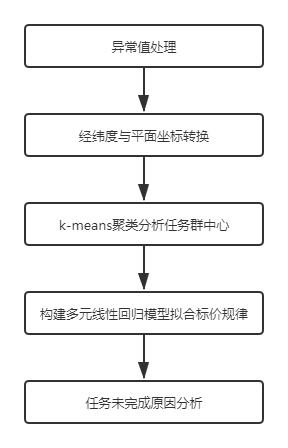
\includegraphics[width=8cm]{../../img/12.png}
% 	\caption{问题一流程图}
% \end{figure}

\subsection{问题二分析}
问题二可以分为三步进行逐一求解。首先分析销售总量与成本加成定价的关系;其次对蔬菜各品类未来一周的销售水平、批发价格进行预测;最后综合销售总量与定价的关系分析结果以及未来一周的预测结果,构建收益最大化决策模型进行求解。其中需要注意的是,销量总量与成本加成定价可能受多种因素的影响,需要建立合适的模型刻画定价与销量的关系。

\subsection{问题三分析}
问题三是混合多目标规划问题。尽管题中要求在满足需求量的前提下进行最大收益优化,但是由于单品数量的限制,无法完全满足顾客的购买需求,因此本题应为一个多目标优化类问题,应对顾客需求满足程度与收益情况进行综合优化。但其中需要注意的是顾客的需求度并不能完全简单地与销售量对等,需寻找评价指标综合销量与销售次数等其他因素,得到需求度。此外需要选择合适的优化算法方能求解。

\subsection{问题四分析}
问题四是一个较为开放的问题,可以根据前三问数据分析结果、处理信息时遇到的难点、实际生活经验并结合相关专业领域文献寻找对商超决策有利的其他数据。

\section{模型的假设}

\begin{itemize}
	\item 假设短期内商超的进货与售价不会对顾客忠诚度造成影响;
	\item 假设短期内,历史售价等客观因素不会对顾客当日需求量造成影响。
	\item 假设商超在这三年中的补货与定价策略已经一定程度上考虑了顾客消费需求;
	\item 该商超附近无其他竞争对手,不存在由恶意竞争引起的销量波动
\end{itemize}

\section{符号说明}

% \usepackage{tabularray}
\begin{table}[h]
	\centering
	% \caption{cap1}
	\begin{tblr}{
	  cells = {c},
	  vline{3} = {-}{},
	  hline{1-2,13} = {-}{},
	}
	符号          & 意义          & 符号           & 意义              \\
	\textit{Qi} & 品类 i 的总销量   & \textit{Qij} & 品类 i 中单品 j 的销量  \\
	\textit{Pi} & 品类 i 的平均定价  & \textit{Pij} & 品类 i 中单品 j 的定价  \\
	\textit{Li} & 品类 i 的平均损耗  & \textit{Lij} & 品类 i 中单品 j 的损耗  \\
	\textit{Bi} & 品类 i 的总补货量  & \textit{Bij} & 品类 i 中单品 j 的补货量 \\
	\textit{Ci} & 品类 i 的补货成本  & \textit{Cij} & 品类 i 中单品 j 的成本  \\
	\textit{wi} & 品类 i 的平均加成率 & \textit{wij} & 品类 i 中单品 j 的加成率 \\
	\textit{M}  & 总销售额        & \textit{T}   & 总成本             \\
	\textit{wi} & 品类 i 定价的加成率 & \textit{wij} & 品类 i 中单价 j 的加成率 \\
	\textit{k}  & 损耗折扣率       & \textit{Dj}  & 需求度             \\
	\textit{Ep} & 需求价格弹性      & \textit{Ec}  & 交叉弹性弹性          \\
	\textit{Ev} & 价格预期弹性      & \textit{EV}  & 交叉弹性弹性          
	\end{tblr}
	\end{table}


\section{数据预处理}

\begin{figure}[H]
	\small
	\centering
	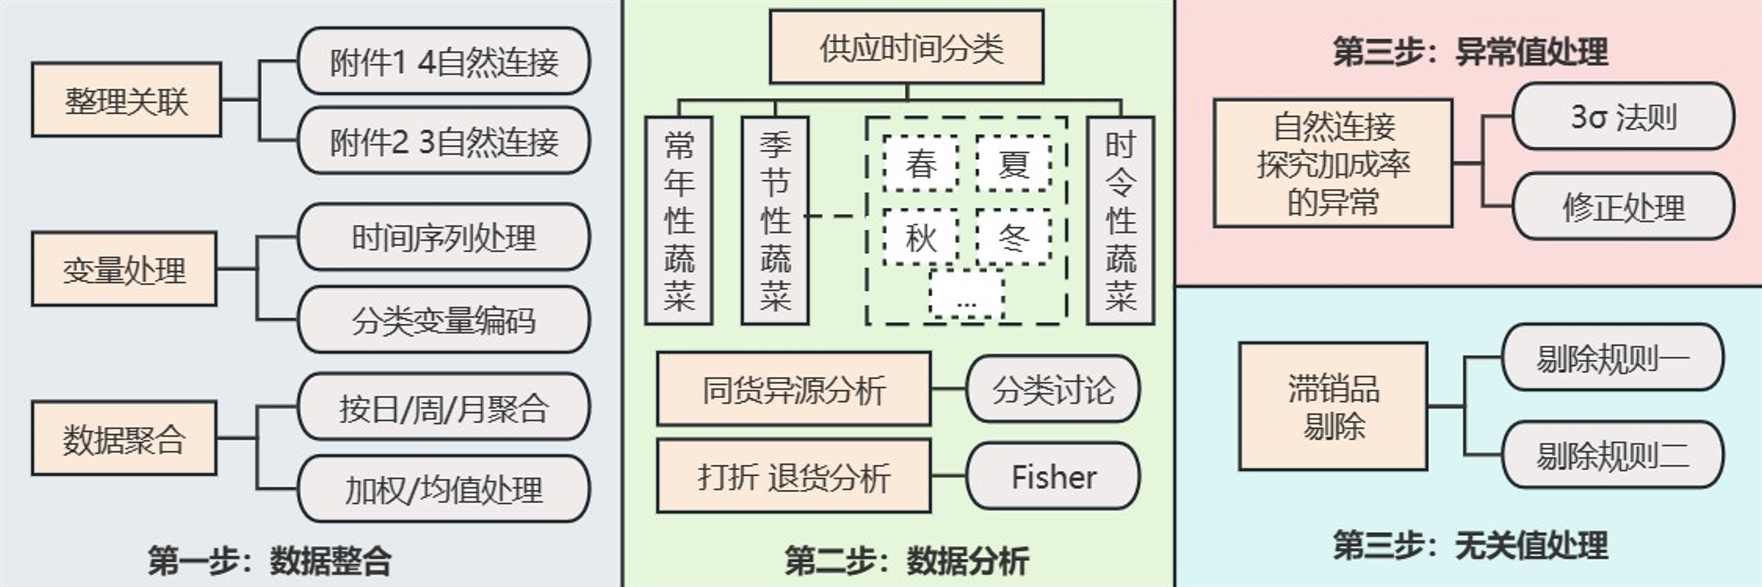
\includegraphics[width=15cm]{../../img/1.png}
	% \caption{任务分布图}
\end{figure}

\subsection{数据整合}

概览题设所给出的附件信息,可以发现其数据量庞大、信息冗杂琐碎,是典型的实际生活数据。对其进行整理关联、变量处理、数据聚合等初步工作能有效帮助后续数据的处理、分析与预测。

\begin{itemize}
    \item \textbf{整理关联}:附件一、四共同描述了单品的编号、分类、近期损耗率信息,而附件二、三共同描述了单品的销售、进购信息,通过 Python 编程以实现表格间自然连接(NJ)。
    \item \textbf{变量处理}:将附件中的列“销售日期”与“销售时间”处理为时间序列、“销售类型”与“是否打折销售”one-hot 编码处理为分类变量。
    \item \textbf{数据聚合}:由于蔬菜单品的销售信息琐碎,故将其以单品和品类两种形式按日、周、月、年进行数据聚合,以品类的日聚合为例介绍聚合规则如下:
    \begin{enumerate}[label=(\alph*)]
		\item 对于日销售量:
		\begin{equation}
			Q_i=\sum_j^{}{Q_{ij}}
		\end{equation}
		其中 Ok 表示每个订单的单品编号,Ai 表示品类i 中的单品集合,Qij 表示品类i 中的单品 j 的销量,Qi 表示品类 i 的总销量
		\item 对于日销售单价、进价、加成率:
		\begin{equation}
			X_i=\frac{\sum_j^{}{Q_{ij}\times x_i}}{Q_i}
		\end{equation}
		其含义可以理解为以销量为权重进行加权求均值,其中加成率的计算公式如下:
		\begin{equation}
			\text{加成率}=\frac{\text{定价}-\text{成本}}{\text{成本}}
		\end{equation}

	\end{enumerate}


\end{itemize}

\subsection{数据分析}

\begin{enumerate}[label=(\alph*)]
    \item 单品按时间供应分类
    \item 同货异源类蔬菜的分析
    \item 打折单品与退货单品分析
    如图2, 对两者进行 Fisher 精确性检验可以发现p 值小于 0.05,说明两者存在相关关系,具体来说即,当打折销售时退货的概率会降低。
\end{enumerate}

\subsection{异常数据处理}

将附件自然连接之后能发现不易被发现的异常数据,如加成率(利润率)。大部分单品的加成率为 0.5 左右,然而存在部分单品加成率高达 200,显然不符合蔬菜一般定价规律。本文对附件二中的 87 余条销售记录进行如下处理:
\begin{itemize}
    \item 3σ 法则:剔除利润率偏差极大的数值
    \item 修正处理:将利润率大于 2 的销售记录剔除
\end{itemize}\

经过处理之后,删去 16430 条销售记录,对商品加成率画出分布图如图3所示。


\subsection{无关数据处理}

观察蔬菜销售数据发现,部分蔬菜在供应上未呈现周期规律性,并且供应天数极少销售量同样极少。本文认为该类蔬菜可能为某段时间突然出现的特殊品种蔬菜,存在供应链不稳定,或者市场需求量极少的情况,并不存在稳定销售以及供应规律,在数据分析中属于无关数据,对蔬菜总销量以及未来预测无有利贡献,因此本文不予进行考虑。本文对无关数据进行如下处理:
\begin{itemize}
	\item 剔除完全没有销量数据的蔬菜单品,共计 5 个;
	\item 剔除销售天数小于 10,销售量小于 3‰,且无年周期规律的蔬菜单品,共计 48 个。
\end{itemize}

\section{问题一的模型建立与求解}

%参考文献
\bibliographystyle{unsrt}
\bibliography{reference}






\newpage
%附录
\begin{appendices}
	\section{墨卡托投影法}
	\begin{lstlisting}[language=matlab]
function [x,y]=ll_xy(lng, lat)
earthRad = 6378137.0;
x = ((lng .* pi) ./ 180) .* earthRad;
a = (lat .* pi) ./ 180;
y = (earthRad ./ 2) .* log((1.0 + sin(a)) ./ (1.0 - sin(a)));
end

tic
format long g
[x_p ,y_p] = ll_xy(x,y);
x_p = x_p - mean(x_p);
y_p = y_p - mean(y_p);
toc
 \end{lstlisting}

	\section{Kmeans-聚类算法}
	\begin{lstlisting}[language=matlab]
opts = statset('Display','final');
%调用 Kmeans 函数
%X N*P 的数据矩阵
%Idx N*1 的向量,存储的是每个点的聚类标号
%Ctrs K*P 的矩阵,存储的是 K 个聚类质心位置
%SumD 1*K 的和向量,存储的是类间所有点与该类质心点距离之和
%D N*K 的矩阵,存储的是每个点与所有质心的距离;
[Idx,Ctrs,SumD,D] = kmeans(X,4,'Replicates',2,'Options',opts);
%画出聚类为 1 的点。X(Idx==1,1),为第一类的样本的第一个坐标;X(Idx==1,2为第二类的样本的第二个坐标
plot(X(Idx==1,1),X(Idx==1,2),'r.','MarkerSize',14)
hold on
plot(X(Idx==2,1),X(Idx==2,2),'b.','MarkerSize',14)
hold on
plot(X(Idx==3,1),X(Idx==3,2),'g.','MarkerSize',14)
hold on 
plot(X(Idx==4,1),X(Idx==4,2),'y.','MarkerSize',14)
%绘出聚类中心点,kx 表示是圆形
plot(Ctrs(:,1),Ctrs(:,2),'kx','MarkerSize',14,'LineWidth',4)
%legend('Cluster 1','Cluster 2','Cluster3','Centroids','Location','NW')
Ctrs
SumD
 \end{lstlisting}

	\section{层次聚类法}
	\begin{lstlisting}[language=python]
import pandas as pd
import seaborn as sns  # 用于绘制热图的工具包
from scipy.cluster import hierarchy  # 用于进行层次聚类,话层次聚类图的工具包
from scipy import cluster
import matplotlib.pyplot as plt
from sklearn import decomposition as skldec  # 用于主成分分析降维的包

from scipy.cluster.hierarchy import dendrogram, linkage, fcluster
from matplotlib import pyplot as plt

df = pd.read_excel("tempdata.xlsx", index_col=0, header=None)  #index_col=0指定数据中第一列是类别名称,PS:计算机程序一般从整数0开始计数,所以0就代表第一列
# df = df.T    #python默认每行是一个样本,如果数据每列是一个样本的话,转置一下即可

X = df.index
# print (X)
# method是指计算类间距离的方法,比较常用的有3种:
# single:最近邻,把类与类间距离最近的作为类间距
# average:平均距离,类与类间所有pairs距离的平均
# complete:最远邻,把类与类间距离最远的作为类间距
Z = linkage(X, 'average')
f = fcluster(Z, 4, 'distance')
fig = plt.figure()
dn = dendrogram(Z)
plt.show()

 \end{lstlisting}
\end{appendices}

\end{document}